\documentclass{article}

\usepackage[
  paperheight=8.5in,
  paperwidth=5.5in,
  left=10mm,
  right=10mm,
  top=20mm,
  bottom=20mm]{geometry}
\usepackage[utf8]{inputenc}

\usepackage{graphicx}
\usepackage{wrapfig}
\usepackage[bottom]{footmisc}
\usepackage{listings}
\usepackage{enumitem}

\usepackage{wrapfig}
\usepackage{ragged2e}

\usepackage{array}
\usepackage[table]{xcolor}
\usepackage{multirow}
\usepackage{booktabs}
\usepackage{hhline}
\definecolor{palegreen}{rgb}{0.6,0.98,0.6}

\usepackage{amsmath}
\usepackage{amssymb}
\usepackage{multicol}
\usepackage{lipsum}
\usepackage{hyphenat}
\PassOptionsToPackage{hyphens}{url}
\usepackage{url}

\usepackage{rotating}

%\usepackage{xeCJK}

%% support use of straight quotes in code listings
\usepackage[T1]{fontenc}
\usepackage{textcomp}
\usepackage{listings}
\lstset{upquote=true}

%% for shrinking space between lines
\usepackage{setspace}

\newcommand*{\affaddr}[1]{#1} % No op here. Customize it for different styles.
\newcommand*{\affmark}[1][*]{\textsuperscript{#1}}
\newcommand*{\email}[1]{\small{\texttt{#1}}}
\newcommand{\tarot}{\textsc{Tarot}}
\renewcommand*\contentsname{\centering Table of Contents}

\renewcommand{\footnoterule}{%
  \kern -3pt
  \hrule width \textwidth height 0.5pt
  \kern 2pt
}

% remove date
\date{}

\usepackage{titlesec}
\titleformat*{\section}{\large\bfseries}
\titleformat*{\subsection}{\normalsize\bfseries}
\titleformat*{\subsubsection}{\normalsize\bfseries}


\usepackage{graphicx}
\usepackage[framemethod=TikZ]{mdframed}
\usepackage{tikz,pgfplots}
\mdfdefinestyle{MyFrame}{%
    linecolor=blue,
    outerlinewidth=2pt,
    roundcorner=20pt,
    innertopmargin=\baselineskip,
    innerbottommargin=\baselineskip,
    innerrightmargin=20pt,
    innerleftmargin=20pt,
    backgroundcolor=white}
\mdfsetup{font=\small}
\usepackage{adjustbox}


\title{A Course-based Undergraduate Research Experience (CURE) in Computer Science: An Experience Report\footnote{\protectCopyright \copyright 2018 by the Consortium for Computing Sciences in Colleges.
Permission to copy without fee all or part of this material is granted provided
that the copies are not made or distributed for direct commercial advantage,
the CCSC copyright notice and the title of the publication and its date appear,
and notice is given that copying is by permission of the Consortium for
Computing Sciences in Colleges.  To copy otherwise, or to republish, requires
a fee and/or specific permission.
}
}

% Target typesetting:
%
%  Baochuan Lu, Author A, John Meinke, Author B
%        Computer and Information Sciences
%          Southwest Baptist University
%               Bolivar, MO 65613
%            {blu,author}@sbuniv.edu
%          Computer Science Department
%              Another University
%              Our Town, TX 00000
%           {jmeinke,author}@univ.edu

\author{
Fahmida Hamid\\
Computer Science\\
Grinnell College\\
Grinnell, IA 50112\\
\email{fahmida.hamid@gmail.com}\\
}

\begin{document}
\maketitle

\begin{abstract}
This article demonstrates a pedagogy of a research-focused Computer Science course for undergraduates in a liberal arts environment. The long term benefits of Course-based Undergraduate Research Experiences (CUREs) in different STEM fields are the driving forces for modeling such a course. The course balances a research-focused, semi-supervised, active learning experience and a traditional lecture-focused, supervised classroom-environment. This article summarizes the current semester's student experiences and suggests possible scope for improvements.
\end{abstract}

\section{Introduction}
Course-based undergraduate research experiences (CUREs) offer an effective way of integrating research into an undergraduate science curriculum and extending research experiences to a large, diverse group of early-career students~\cite{doi:10.1187/cbe.14-01-0004,doi:10.1187/cbe.18-07-0126}. Students who participate in CUREs develop content knowledge and technical skills specific to the area of research~\cite{10.1093/femsle/fnx157}. An increasing number of well-designed and well-controlled studies show that CUREs can influence students learning, development, and educational and career trajectory\cite{eagan2013making,hurtado2009diversifying,schultz2011patching}. Several studies~\cite{doi:10.1187/cbe.14-01-0004,doi:10.1187/cbe.18-07-0126} discuss about research-focused courses in different STEM fields: Biology, Chemistry, Medicine, etc. In the Computer Science (CS) discipline, though there have been some practice already in different organizations, a model for such course has not yet been reported to the academic community. This article details a model of a CS course following the principles of course-based undergraduate research experience. 
\par In this paper, section~\ref{cureinCS} describes the course structure and activities, section~\ref{stuexp} states student experiences and outcomes, section~\ref{extension} makes suggestions about extending the goals and involvements beyond the classroom, and section~\ref{concl} draws conclusion. Due to the page-limit constraints, detail definition and logical structure of CURE, short and long term benefits of such courses are omitted. Interested readers might find relevant information in article~\cite{doi:10.1187/cbe.14-01-0004}.
   
\section{CURE in Practice for CS Students}
\label{cureinCS}
 In Computer Science, research areas such as Natural Language Processing, Information Retrieval, Machine Learning, Artificial Intelligence, Data Science, etc. do not always need specialized equipments/hardwares other than a modern computer-equipped lab space (teaching-lab) for deploying a full research-focused course. The experience report is based on such course in Information Retrieval(IR) track. The next couple of sections outline the structure and activities of the course.

\subsection{Course Layout}
%The course is a mixed bag of traditional classroom-teaching model and research-focused active learning model as it is important to teach the students some topics and train them through some activities to get ready for conducting the research. 
The course objective is to provide hands-on experiences with several existing software tools through the programming assignments and to train them to develop critical thinking and analytical skills through written assignments. In order to offer a balanced way of learning new techniques and applying them for conducting research, the course is divided into two main phases: 
\begin{itemize}
\item Supervised Learning Phase
\item Semi-supervised Learning (Research) Phase
\end{itemize}
The next two sections introduce the major activities during these phases.

\begin{figure}[h]
\centering
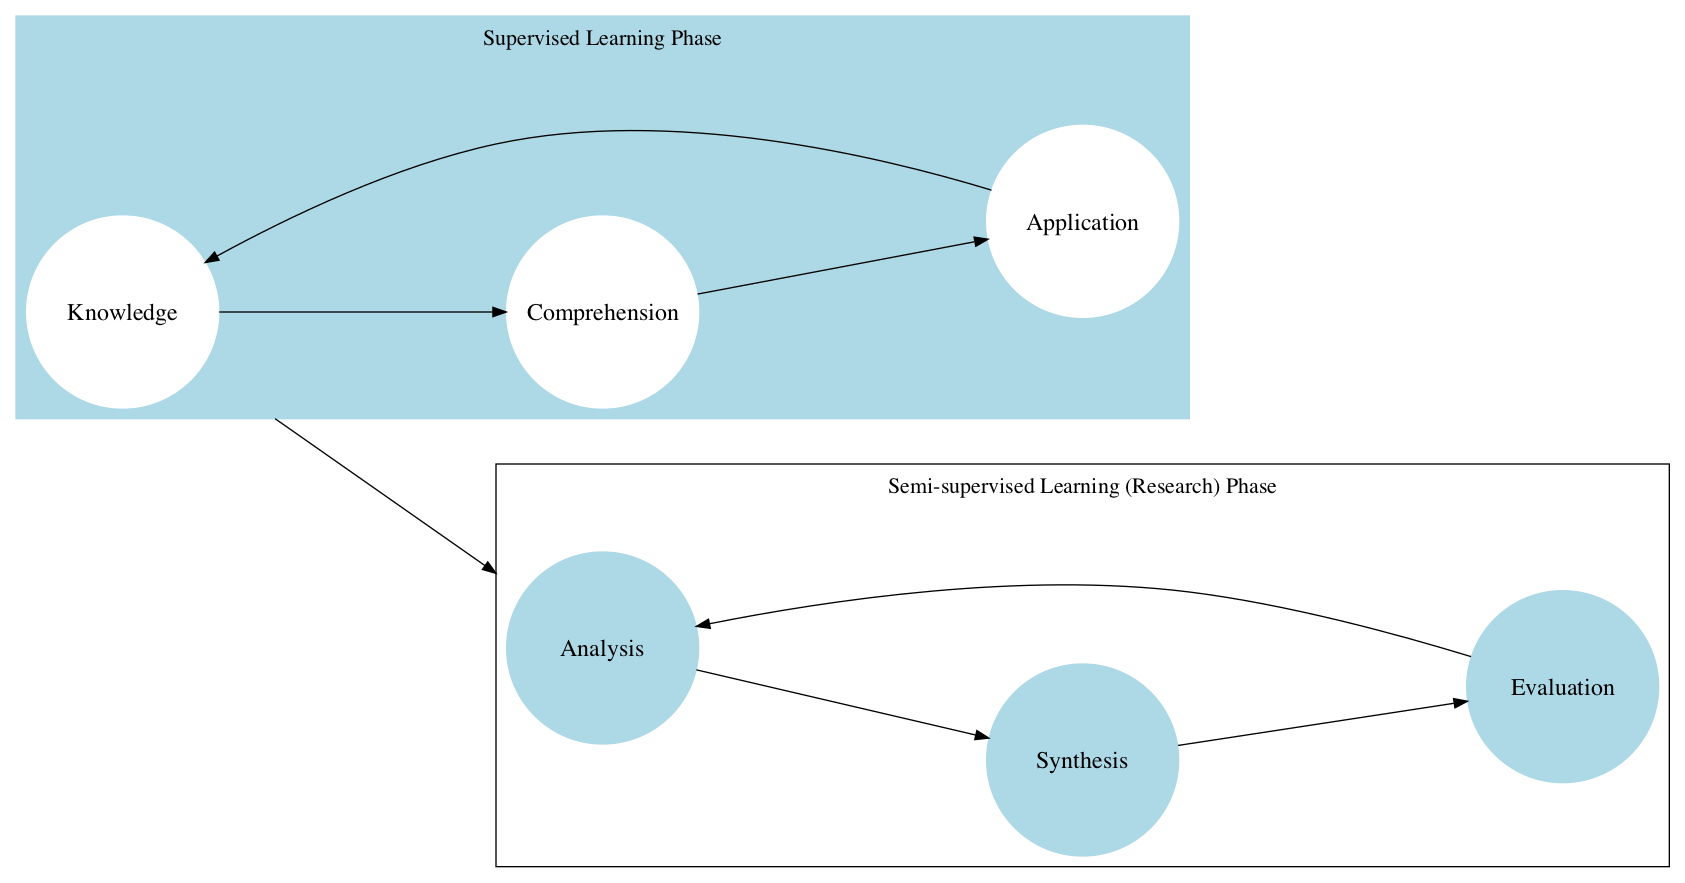
\includegraphics[width=.75\textwidth]{./figures/graph2}
\caption{A revised Bloom's Taxonomy~\cite{adams2015bloom} for a research-focused course.} \label{fig1}
\end{figure}

\subsection{Supervised Learning Phase (Week 1 $\sim$ Week 7)}
The activities of this phase are mostly {\bf lectures} highlighting and demonstrating important concepts from textbook readings. When appropriate, external readings can be used. Students are asked to complete written assignments (individual works), in-class tasks and programming assignments (group works). 
\subsubsection{In-Class Tasks}
Providing students with models and worked examples can help them learn to solve problems faster~\cite{rosenshine2012principles}. During the second hour of every class, students either run/test small experiments (with code provided by the instructor) or implement/modify a partially solved model to get a better understanding. 


\subsubsection{Programming Assignment}
The programming assignments are designed with the following goals in mind:
\begin{itemize}[noitemsep, nolistsep]
\item Students should have a lot of freedom in choosing the layout and the techniques while implementing the solution. %In a research-focused course, this is an important step as  the final goal is to train them to discover new and better techniques on their own. 
\item Students should know about the standard evaluation techniques and be able to design new scales of measures.
\item Students should write detailed reports for the experiments. 
\item Students should be comfortable using different standard datasets so that they can test their work with larger collections.
\end{itemize}
\subsubsection{Written Assignment}
Students are asked to submit written reports (summarize the concepts and answer few related questions) about published articles (chosen by the instructor) during the first and the fourth week. The goal is to improve their analytical and writing skills on technical matters.
\par Programming assignments and the template for written assignments can be found in appendix~\ref{appA}. 

\subsubsection{Term Exam} 
The supervised learning phase ends with an open-book, two-hour long exam where students are asked to solve analytical questions on covered topics.
\par The covered topics on this phase can be found in appendix~\ref{appB}. 
\subsection{Research Phase (Week 8 $\sim$ Week 14)}
The first day of this phase is a full lecture led by the instructor introducing the students to different research sub-areas and possible research problems in each of those areas. At the end of the session, students form groups on their own and start talking about possible research problems that sound interesting to them.
\begin{figure}[h]
\centering
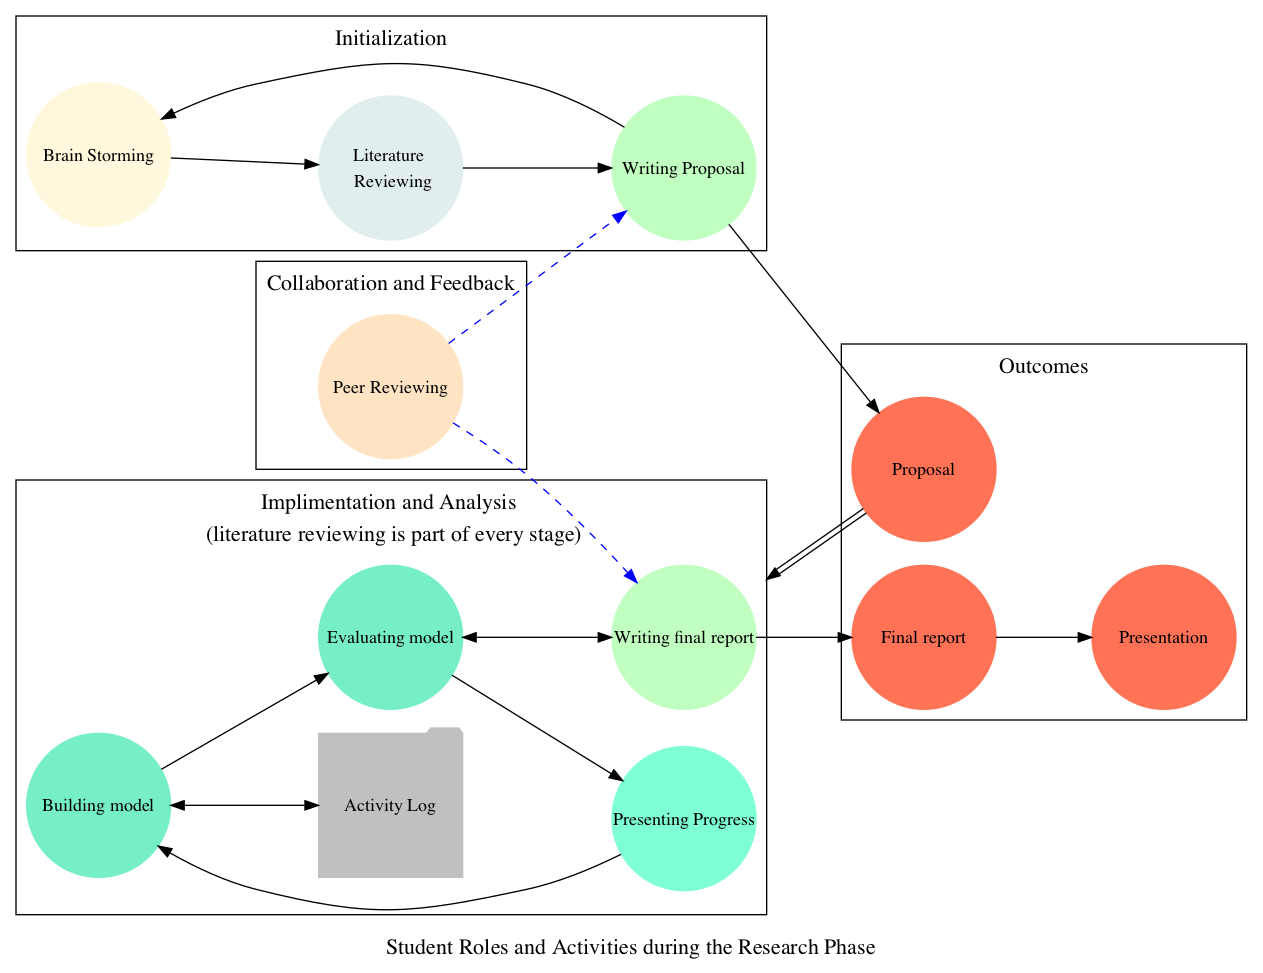
\includegraphics[width=.75\textwidth]{./figures/graph3}
\caption{Major Student Activities during the Research Phase} \label{fig2}
\end{figure}
\par The instructor takes a passive role (monitor and guide) from now on. During the eighth week, students spend their time on writing research proposals which are approved after two trials of presentation (one informal and one formal) in front of the class. 
\par As {\bf literature reviewing} is an important part of research, each student-group presents two articles (relevant to their research idea) as a basis of their work. They also submit a weekly plan: approximate amount of spent time per week and tentative weekly goal. Asking them to budget time is important as this helps them find a balance between their ambitions and achievable goals within time and other constraints. Based on the demand of the research project, students may need to find relevant datasets or state a plan for creating datasets. 
\begin{mdframed}
{\bf Template/Guideline for Writing A Research Proposal}
\begin{description}
\item [Title:] Find an interesting and representative title.
\item [Abstract:] Highlight the basic idea and its importance.
\item [Project Description:] With few literature reviews, explain your idea, the scope, the broader impact of your project.
\item [Datasets:] Cite proper existing datasets (if required) that you plan to use or explain how you plan to construct one for your work. 
\item [Preparation:] Report the skills and knowledge that you think will be useful.
\item [Outcomes \& Timeline:] Highlight some final expected outcomes (a paper, poster, software, API, etc.)
\item [References:] Cite relevant research works (at least 5 to begin with).
\end{description}
\end{mdframed}
\par To make the students accountable for maintaining the quality of their work, every student also work as {\bf anonymous reviewer} for other students' projects. The final work is  submitted as a paper following standard formats commonly found in most technical IR articles: title, abstract, introduction, related work, dataset, methodology, result analysis, and conclusion/future directions.

\begin{mdframed}
{\bf Review Template}
\begin{enumerate}
\item Summarize the project-idea in your own words.
\item Rate at the scale of 1 to 10 (1 being the worst and 10 being the best):
	\begin{itemize}
	\item Is the research question clearly stated?
	\item Have they explained clearly why their idea is interesting and impactful to some parties?
	\end{itemize}
\item State some strengths and some weaknesses of the project idea.
\item Have they clearly talked about the evaluation mechanism and datasets (if needed) for their project?
\item (Optional) Provide some suggestions to the team. 
\end{enumerate}
\end{mdframed}


\par Careful attention is paid on their {\bf writing quality}: explaining the methodology and contribution, citing relevant works, acknowledging peers for their comments and suggestions, etc. The 14-week long activity ends with formal 20-min presentation by each group in a seminar hall where students from the school will be invited to attend.

\subsection{Time Commitment}

\par The students meet twice a week for 2 hours in a teaching lab. It is expected from the students that they would complete assigned readings (approximately 1$\sim$2 hours) for the class and complete the assignments outside of class-meetings (approximately 4$\sim$6 hours). Overall, students are expected to spend approximately 7$\sim$10 hours per week for the course.

\subsection{Grading/Assessment}
50\% of the course grade is allocated for the research phase. Clarity of thinking, efficiency of implementation, depth of analysis, structure and readability
of the project report, and final presentations are the determining factors for achieving that 50\% score. The rest of the course-grade is distributed on regular programming assignments, written assignments, class participation, and one term exam.

\section{Students Experiences}
\label{stuexp}
Given the research sub-areas as \{Keyphrase extraction and Summarization, Learning to rank, Question-Answering, Recommender Systems\}, the running student projects are the followings:
\begin{mdframed}[style=MyFrame, frametitle={Student Projects}]
\begin{description}
\item [Information Desk:] to create a powerful Question-Answering system, leveraging the power of Generative Adversarial Networks (GAN) and the World Wide Web (WWW).

\item [Teaching Machines:] to Reason on texts, to build a Question-Answering model with complex questions (how or why) and eventually understand the sequential facts embedded in the documents to produce the answer.

\item [Keyphrase Extraction of YouTube Video Transcripts:] to outline the contents and to create tags to improve search results.

\item [A Study of Keyphrase Extraction on Celebrity Tweets:]  to create a celebrity-tweet dataset and apply unsupervised keyphrase extraction techniques on it. 
\end{description}
\end{mdframed}

\par The first two groups are studying several Machine Learning techniques for implementing automatic answer generation in different situations. The third group is using YouTube's API for building their own ``transcript dataset'' and applying meta-information to build a Naive-Bayes Classifier for extracting meaningful phrases. The fourth group has manually created a dataset of ``Monthly Celebrity-tweets'' and will be using an unsupervised technique to automatically extract keywords. The first and the third group will use human annotators to help create gold-standards for evaluating their system's performances. The second group uses a dataset published by Facebook that comes with standard answers. The group plans to extend the model from producing short phrased answers to a complete sentence. 
\par The major outcomes of the course from the student perspectives are: 
\begin{enumerate}[label=(\alph*), noitemsep, nolistsep]
\item To be able to write a research proposal and a technical paper.
\item To be able to think independently and discover a problem (area of concern) 
\item To be able to write constructive criticisms of other's work.
\item To plan for publishing the work as a student paper/poster to a proper venue.  
\end{enumerate}
%The course is well accepted by majority of the enrolled students of the class. The pedagogy initially sounded intimidating and unusual to few of them but they eventually acknowledged that the heavy-weight programming assignments were necessary to help them push their programming and analytical skills up to a higher level. Also, all the students appreciated that having a course where they can spend/invest more than two weeks on building/solving their own research idea is actually helpful for them to experience {\bf the path of scientific discovery}. 
\section{Extending the Scope and Possibilities}
\label{extension}
If planned with enough time and resources, several other possibilities can be included to add more value and learning experience:\\

\par {\bf Invited talks: } Scholars in similar research tracks can occasionally give invited-talks. In some cases, students can remotely join at different events (e.g. ACM TechTalk) and thus flip a lecture on similar/same topic.
%Scholars in similar research tracks occasionally give invited-talks. Faculty has to figure out if that can be a possibility given the support from the organization and the potential speakers interest and timeframe. Not only students from the class but also a larger body of the students can be benefitted from such events. In some cases, students can remotely join at different events (e.g. ACM TechTalk) and thus flip a lecture on similar/same topic.\\

\par {\bf Student talks: } Offering bonus-points for actively participating in some student clubs and presenting the research will help students build confidence and acquire more knowledge. This can motivate the students in audience seats for conducting research as well.

\par {\bf Workshop/Poster presentations: } Students should aim for presenting their work to external events. Regional or national undergraduate research symposiums are possible suits for their work.``What will be the impact of my research?'', ``Why is this problem still unsolved?'' -- these questions lead students into determining the scale of their work and not limit their achievements only to a good letter grade.

%In a research-focused course, it is important to set a final achievable goal to the students which can be, for example, presenting the final work to a weekly event at the department or even to a larger audience. This not only helps building their confidence but also enforces them in thinking about a goal-oriented research. ``Who will be benefitted from my work?" or ``What will be the impact of my research?", ``Why is this problem still unsolved or so challenging?" -- these questions lead students into determining the scale of their work and not limit their achievements only to a good letter grade. 
%\par As the students are not aware of all these scholarly activities, the faculty needs to keep motivating the students time-to-time by informing them about relevant events (deadlines, formats, etc.) Students can use these workshops or presentation events as a way for building networking opportunities.
%%% for example, the groups of students are aiming to present their work as posters to upcoming CCSC-MidWest or CCSC-Central Plain conferences.


\section{Conclusion}
\label{concl}
The goal of the course is to lead the students to the process of scientific discovery in a small scale. The first round of experiment at Grinnell College with eight senior students has been successful in several ways. Given more time and scope, in next trial, several modifications can be done: having an overlapping research and supervised learning phase, offering student-stipends for teams that can participate at poster/workshop events outside of the college, etc. In short, research-focused courses create a trend of involving undergraduates into research in an effective way. Faculties with different research interests should offer research-focused courses by rotation to engage larger and diverse set of students. 

\bibliographystyle{plain}
\bibliography{mybibliography}
%\newpage
\appendix
\section{Sample Assignments}
\label{appA}
\begin{mdframed}[style=MyFrame]
\small
\label{Problem1}
Programming Assignment 01\\
Allocated Time: 2 weeks\\
Goal: To implement one of the most common applications in IR\\
Problem Statement:\\
Build a search engine using your preferred programming language. Your code should be well documented. While implementing your engine, follow the basic building blocks of a standard search engine. Report the strengths and weaknesses of your model.  
\par Server Side should do the followings: crawl at least 100 unique pages, parse them, create index, build web-graph by analyzing the links, and rank them (you may want to implement the page-rank algorithm). It is a good idea to design a topical search engine, like, crawl pages whose title contains a particular topic (e.g. sports). That way, your web-graph will be well-connected. Client Side should have a very simple interface to take input (text query) from the user, search in the index, and print the related web-links in some order. Bonus points will be allocated for designing interactive user-interfaces.  
\end{mdframed}


\begin{mdframed}[style=MyFrame]
\label{Problem2}
\small
Programming Assignment 02\\
Allocated Time: 2 weeks\\
{\bf Goal:} To find the latent features from the so-called unstructured and abnormally large collection of data.\\
Problem Statement:\\
The spam filtering problem is one kind of text categorization problem with the categories being spam and ham. The structure of email is richer than that of flat text, with meta-level features such as the fields found in MIME compliant messages. Researchers have recently acknowledged this, setting the problem in a semi-structured document classification framework. Several solutions have been proposed to overcome the spam problem. Among the proposed methods, much interest has focused on the machine learning techniques in spam filtering. They include rule learning, Naive Bayes, decision trees, support vector machines, or combinations of different learners. The basic and common concept of these inductive approaches is that using a classifier to filter out spam and the classifier is learned from training data rather than constructed by hand. 
\par Your job is to choose two possible machine learning approaches to solve the problem and analyze their performances. Then you will report possible mechanisms to improve the current models you implemented.
\end{mdframed}
\begin{mdframed}[style=MyFrame]
\label{Problem3}
\small
Written Assignment\\
Allocated Time: 1 week\\
Study a given article ``ABC" and answer the following questions:\\
\begin{itemize}
\item Summarize the article. (State the overall contribution of the article within 500 words.)
\item Explain their hypothesis using the following structure: (assume a relevant structure M is given.)
\item The authors used mechanism P and Q for evaluation. Suggest another relevant evaluation mechanism.
\item State at least two cases where the stated hypothesis will fail (or, State some weaknesses).
\item Find another problem where you think the hypothesis (solution) can be applied equally effectively.
\end{itemize} 
\end{mdframed}
%\setlength\LTleft{0pt}
%\setlength\LTright{0pt}
\section{Covered Topics}
\label{appB}

\begin{table}[h]
\centering
%\caption{Tentative Schedule for 8 Weeks}
%\label{my-label}
\small
\begin{tabular}{|l|}
\hline
 Topics Covered \\\hline

         Boolean Retrieval Model \\
         Search Engine Architecture\\
	     Web Crawler \& Basic Text Processing Technique\\
         Inverted Index \& Query Processing \\
	     Search Result Interface \& Link Analysis\\
	     Vector Space model \\
	     Probabilistic Information Retrieval\\
	     Language Models\\
         Evaluation in IR\\
	     Discussion on possible Research Tracks \\
	      - Question-Answering\\
	      - Recommender Systems\\
	      - Keyphrase Extraction\\
	      - Learning to Rank\\
	     \hline     
\end{tabular}	      
\end{table}%}

\end{document}
